With the Knowledge Flow interface, users select WEKA components from a
tool bar, place them on a layout canvas, and connect them into a
directed graph that processes and analyzes data. It provides an
alternative to the Explorer for those who like thinking in terms of
how data flows through the system. It also allows the design and
execution of configurations for streamed data processing, which the
Explorer cannot do. You invoke the Knowledge Flow interface by
selecting \textit{KnowledgeFlow} from the choices on the panel shown
in Figure~\ref{subfig:explorer_1}.

\section{Getting started}

\begin{figure}[!th]
\centering
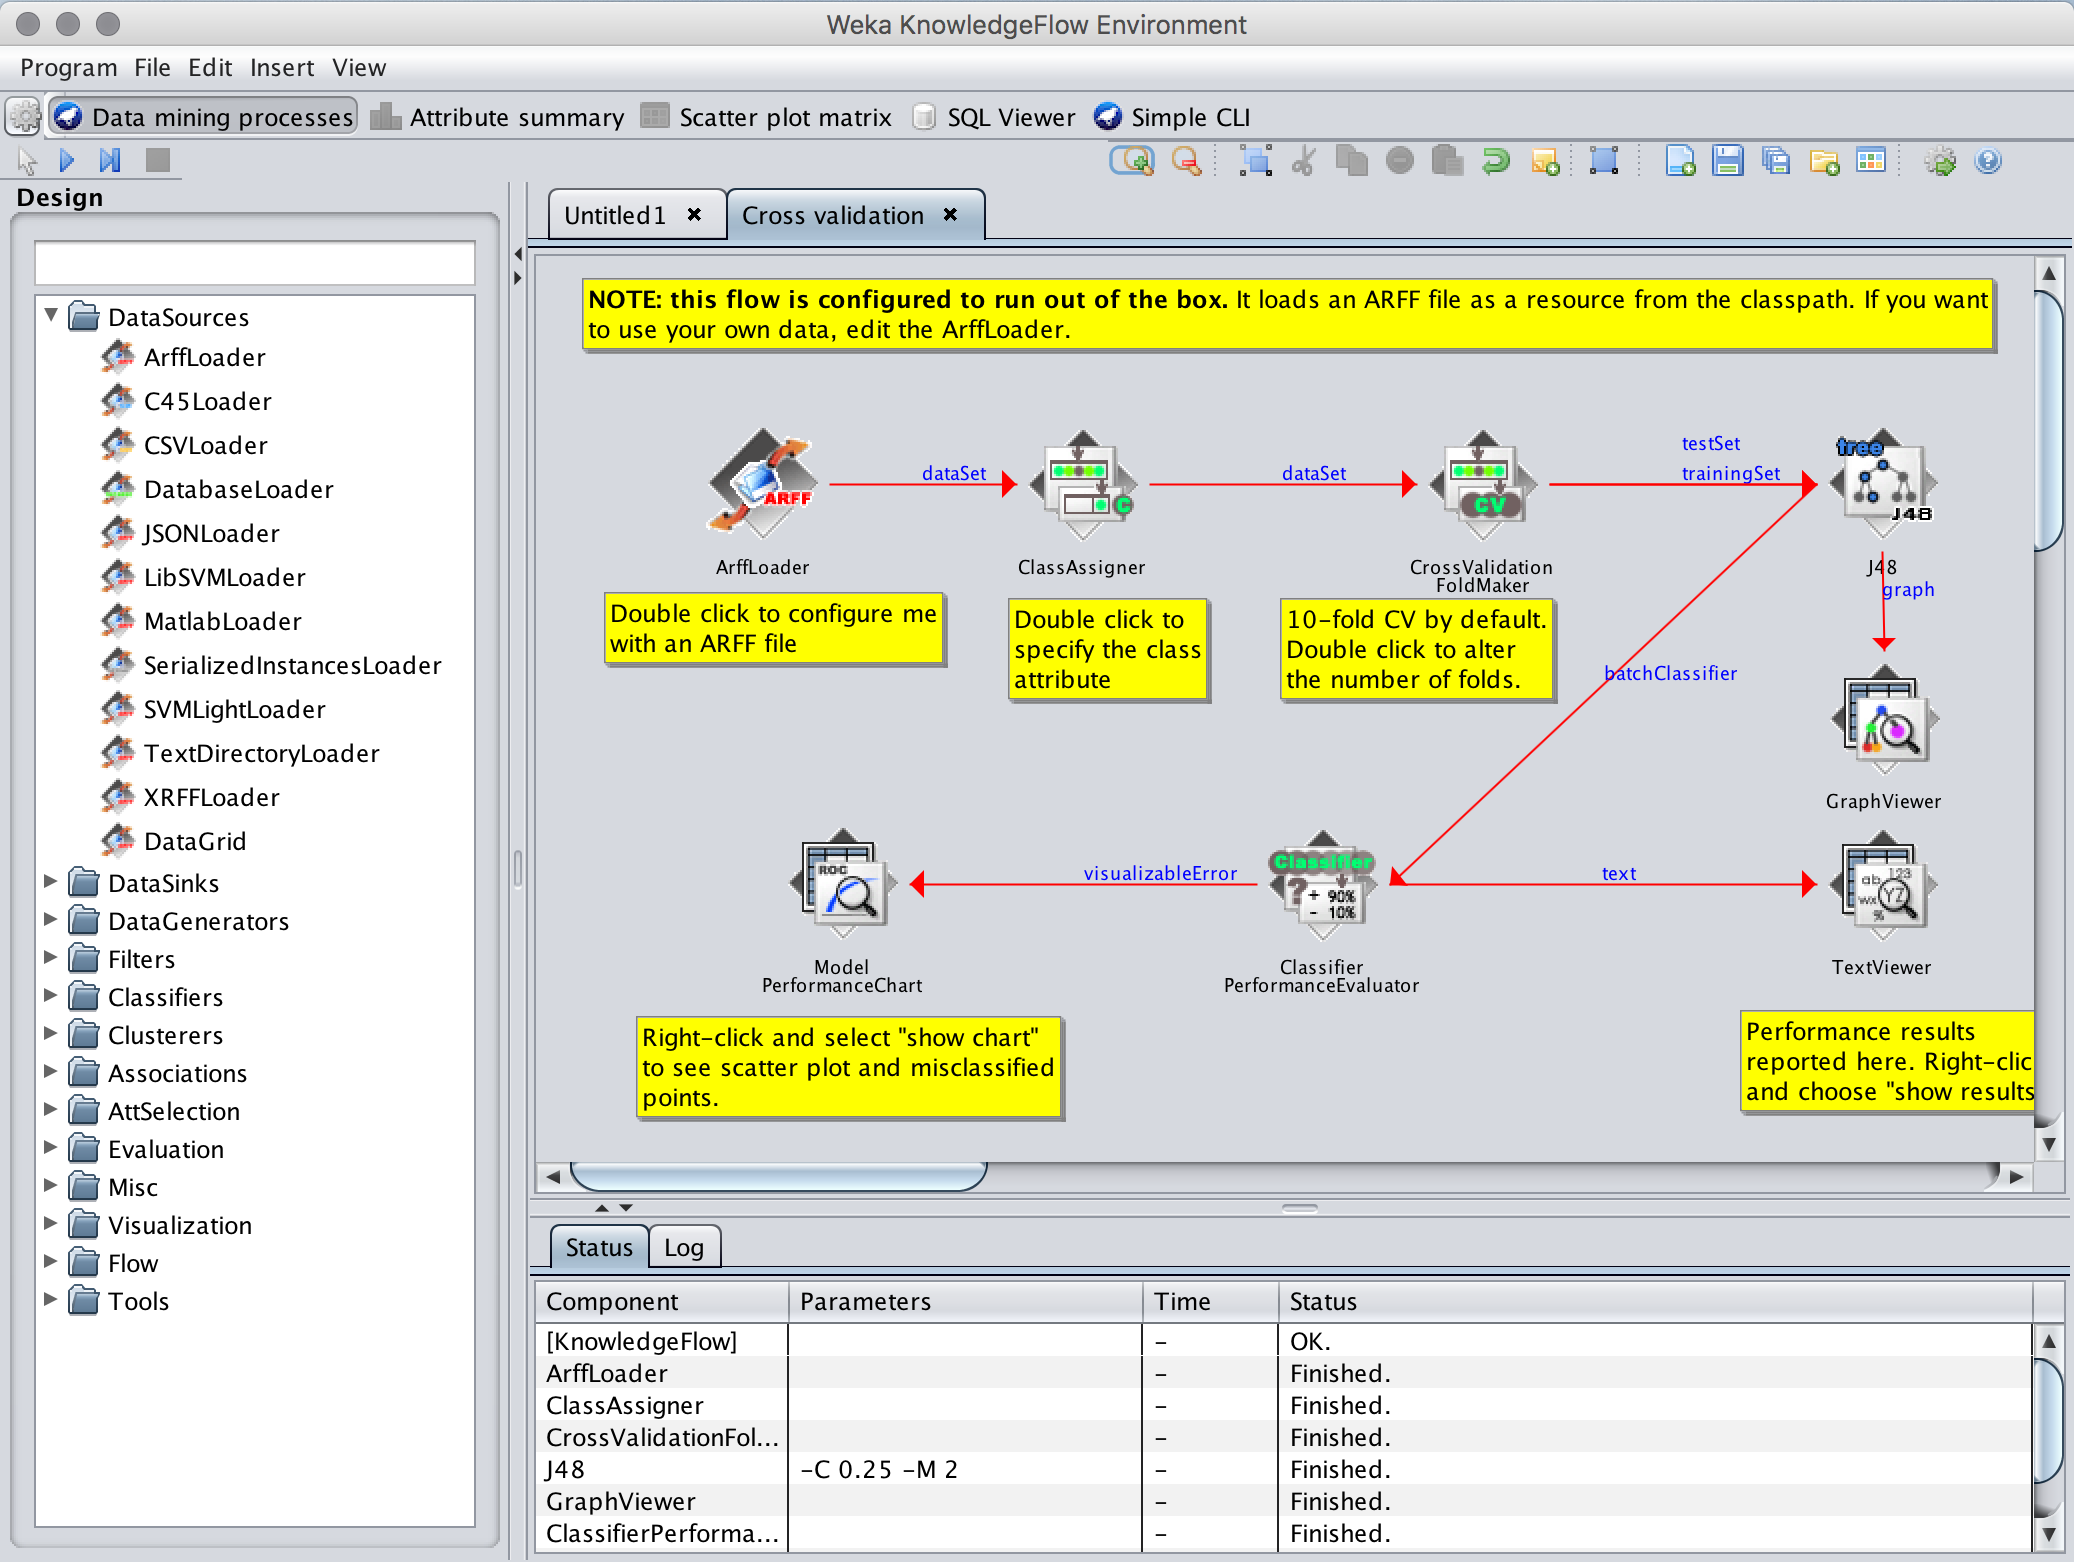
\includegraphics[width=0.95\textwidth]{images/B3_1.png}
\caption{The Knowledge Flow interface.}
\label{fig:knowledge_flow}
\end{figure}

\begin{figure}[!th]
\centering
\subfloat[Right-click menu.]{\label{subfig:arffloader_1}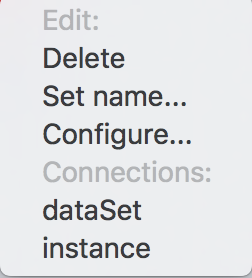
\includegraphics[width=0.25\textwidth]{images/B3_2a.png}}
\qquad
\subfloat[File browser obtained from the \textit{Configure} menu.]{\label{subfig:arffloader_2}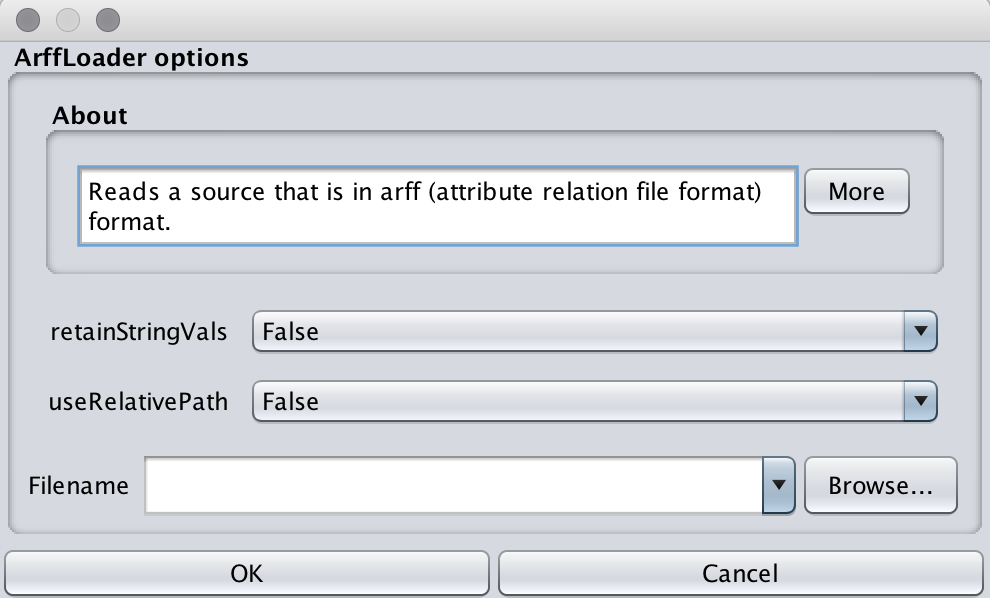
\includegraphics[width=0.65\textwidth]{images/B3_2b.png}}
\caption{\label{fig:kf_arffloader}Configuring a data source in the Knowledge Flow.}
\end{figure}

Here is a step-by-step example that loads an ARFF file and performs a
cross-validation using J48. We describe how to build up the final
configuration shown in Figure~\ref{fig:knowledge_flow}. First create a
source of data by expanding the \textit{DataSources} folder in
the \textit{Design} palette and selecting \textit{ARFFLoader}. The
mouse cursor changes to crosshairs to signal that you should next
place the component. Do this by clicking anywhere on the canvas,
whereupon a copy of the ARFF loader icon appears there. To connect it
to an ARFF file, right-click it to bring up the pop-up menu shown in
Figure~\ref{subfig:arffloader_1}. Click \textit{Configure} to get the
dialog in Figure~\ref{subfig:arffloader_2}, from which you can either
browse for an ARFF file by clicking the \textit{Browse} button, or
type the path to one in the Filename field.

Now we specify which attribute is the class using
a \textit{ClassAssigner} object. This is found under
the \textit{Evaluation} folder in the \textit{Design} pallete, so
expand the \textit{Evaluation} folder, select
the \textit{ClassAssigner}, and place it on the canvas. To connect the
data source to the class assigner, right-click the data source icon
and select dataset from the menu, as shown in
Figure~\ref{subfig:arffloader_1}. A rubber-band line appears. Move the
mouse over the class assigner component and left-click. A red line
labeled dataset appears, joining the two components. Having connected
the class assigner, choose the class by right-clicking it, selecting
\textit{Configure}, and entering the location of the class attribute.

We will perform cross-validation on the J48 classifier. In the data
flow model, we first connect the \textit{CrossValidationFoldMaker} to
create the folds on which the classifier will run, and then pass its
output to an object representing
J48. \textit{CrossValidationFoldMaker} is in the Evaluation
folder. Select it, place it on the canvas, and connect it to the class
assigner by right-clicking the latter and selecting dataset from the
menu (which is similar to that in
Figure~\ref{subfig:arffloader_1}). Next select J48 from the trees
folder under the \textit{Classifiers} folder and place a J48 component on the
canvas. Connect J48 to the cross-validation fold maker in the usual
way, but make the connection twice by first choosing \textit{trainingSet} and
then \textit{testSet} from the pop-up menu for the cross-validation fold
maker. The next step is to select a \textit{ClassifierPerformanceEvaluator}
from the \textit{Evaluation} folder and connect J48 to it by selecting the
\textit{batchClassifier} entry from the pop-up menu for J48. Finally, from the
\textit{Visualization} folder we place a \textit{TextViewer} component on the
canvas. Connect the classifier performance evaluator to it by
selecting the text entry from the pop-up menu for the performance
evaluator.

At this stage the configuration is as shown in
Figure~\ref{fig:knowledge_flow} except that there is as yet no graph
viewer. Start the flow of execution by clicking one of the two
triangular-shaped ``play'' buttons at the left side of the main
toolbar. The leftmost play button launches all data sources present in
the flow in parallel; the other play button launches the data sources
sequentially, where a particular order of execution can be specified
by including a number at the start of the component's name (a name can
be set via the Set name entry on popup menu). For a small dataset
things happen quickly. Progress information appears in the status area
at the bottom of the interface. The entries in the status area show
the progress of each step in the flow, along with their parameter
settings (for learning schemes) and elapsed time. Any errors that
occur in a processing step are shown in the status area by
highlighting the corresponding row in red. Choosing \textit{Show
results} from the text viewer's pop-up menu brings the results of
cross-validation up in a separate window, in the same form as for the
Explorer.

To complete the example, add a \textit{GraphViewer} and connect it to
J48's graph output to see a graphical representation of the trees
produced for each fold of the cross-validation. Once you have redone
the cross-validation with this extra component in place,
selecting \textit{Show results} from its pop-up menu produces a list
of trees, one for each cross-validation fold. By creating
cross-validation folds and passing them to the classifier, the
Knowledge Flow model provides a way to hook into the results for each
fold.

The flow that you've just laboriously created is actually available
(minus the \textit{GraphViewer}) as a
built-in \textit{template}. Example templates can be accessed from the
\textit{Template} button, which is the third icon from the right in the toolbar
at the top of the Knowledge Flow interface. There are a number of
templates that come with WEKA, and certain packages, once installed
via the package manager, add further ones to the menu. The majority of
template flows can be executed without further modification as they
have been configured to load datasets that come with the WEKA
distribution.

\section{Knowledge Flow components}

Most of the Knowledge Flow components will be familiar from the
Explorer. The \textit{Classifiers} folder contains all of WEKA's
classifiers, the \textit{Filters} folder contains the filters,
the \textit{Clusterers} folder holds the clusterers,
the \textit{AttSelection} folder contains evaluators and search
methods for attribute selection, and the \textit{Associations} panel
holds the association rule learners. All components in the Knowledge
Flow are run in a separate thread of execution, except in the case
where data is being processed incrementally---in this case a single
thread of execution is used because, generally, the amount of
processing done per data point is small, and launching a separate
thread to process each one would incur a significant overhead.

Possible data sources are ARFF files, XML ARFF files, JSON ARFF files,
CSV files exported from spreadsheets, the C4.5 file format, databases,
serialized instances, LibSVM and SVMLight data formats, and a special
loader (\textit{TextDirectoryLoader}) to load a directory of plain
text files into a single set of instances. There is also a data source
called
\textit{DataGrid} that allows the user to define attributes and enter the vaues
of instances via a graphical interface. There is a data sink that
corresponds to each data source, with the exception of the
\textit{TextDirectoryLoader} and \textit{DataGrid}. In addition, there are data sinks
that can save raw text, static image data and WEKA serialized models.

Under the \textit{Visualization} folder, the \textit{DataVisualizer}
pops up a panel for visualizing data in a two-dimensional scatter plot
as in Figure~\ref{subfig:j48_4}, in which you can select the
attributes you would like to see. \textit{ScatterPlotMatrix} pops up a
matrix of two-dimensional scatter plots for every pair of attributes,
shown in Figure~\ref{subfig:visualize_1}. \textit{AttributeSummarizer}
gives a matrix of histograms, one for each attribute, like that in the
lower right-hand corner of Figure~\ref{subfig:explorer_2}.\textit{
ModelPerformanceChart} draws ROC curves and other threshold
curves. \textit{CostBenefitAnalysis} allows interactive exploration of
the tradeoffs in cost or benefit arising from different cost
matrices. \textit{GraphViewer}, used above, pops up a panel for
visualizing tree-based models, as in Figure~\ref{subfig:j48_3}. As
before, you can zoom, pan, and visualize the instance data at a node
(if it has been saved by the learning algorithm).

\textit{StripChart} is a new visualization component designed for use with
incremental learning. In conjunction with the
\textit{IncrementalClassifierEvaluator} described in the next paragraph it
displays a learning curve that plots accuracy---both the percentage
accuracy and the root mean-squared probability error---against time. It
shows a fixed-size time window that scrolls horizontally to reveal the
latest results.

Under the \textit{Evaluation} folder, \textit{TrainingSetMaker}
and \textit{TestSetMaker} make a dataset into the corresponding kind
of set. The \textit{CrossValidationFoldMaker} constructs cross-validation folds
from a dataset; the \textit{TrainTestSplitMaker} splits it into training and
test sets by holding part of the data out for the test set. The
\textit{ClassAssigner} allows you to decide which attribute is the class. With
\textit{ClassValuePicker} you choose a value that is treated as the positive
class when generating ROC and other threshold curves. The
\textit{ClassifierPerformanceEvaluator} collects evaluation statistics: it can
send the textual evaluation to a text viewer and the threshold curves
to a performance chart. The \textit{IncrementalClassifierEvaluator}
performs the same function for incremental classifiers: it computes
running squared errors and so on. There is also a
\textit{ClustererPerformanceEvaluator}, which is similar to the
\textit{ClassifierPerformanceEvaluator}. The \textit{PredictionAppender} takes a
classifier and a dataset and appends the classifier's predictions to
the dataset.

Components under the \textit{Flow} folder tend to affect the flow of
data in some way. \textit{FlowByExpression} enables incoming data to
be sent to two downstream components based on the evaluation of a
logical expression. The expression can involve one or more clauses
that test the value of an attribute in the incoming data against a
constant or the value of another attribute. Multiple clauses can be
and'ed or or'ed together. \textit{Block}, when connected between two
components, delays the passing of data to the downstream component
until a user-specified component has finished
processing. \textit{InstanceStreamToBatchMaker} collects instances
arriving in a stream from an incoming ``instance'' connection and
produces a batch dataset when the last instance has arrived. This is
particularly useful when placed after a reservoir sampling filter---it
allows the instances output by reservoir sampling to be used to train
batch learning schemes. The {\em Join} component performs an inner join on
two incoming dataset or instance streams. The user specifies the key
fields to join on for both datasets, and both are expected to arrive
in sorted order of their key fields.

Under the \textit{Tools} folder, \textit{Sorter} sorts instances
within batch datasets or instance streams according to the values of
one or more user-specified attributes. It can handle datasets larger
than can be fit into main memory by using instance connections and
specifying an in-memory buffer size. The component implements a merge
sort by writing the sorted in-memory buffer to a file when full, and
then interleaving instances from the disk-based file(s) when the
incoming instance stream has finished. \textit{SubstringReplacer}
replaces occurrences of substring or regular expression matches in
incoming string attributes with user-specified
values. \textit{SubstringLabeler} matches substrings in a similar
fashion, but instead of replacing them it creates a new attribute in
the data that holds the value of a label specified by the user for
each match condition.

\section{Configuring and connecting the components}

You establish the knowledge flow by configuring the individual
components and connecting them up. The menus that are available by
right-clicking various component types have up to three sections:
\textit{Edit}, \textit{Connections}, and \textit{Actions}. 
The \textit{Edit} operations delete components and open up their
configuration panel. You can give a component a name by
choosing \textit{Set name} from the pop-up menu. Classifiers
and filters are configured just as in the Explorer. Data sources are
configured by opening a file (as we saw previously) or by setting a
database connection, and evaluation components are configured by
setting parameters such as the number of folds for
cross-validation. The {\em Connections} operations are used to connect
components together by selecting the type of connection from the
source component and then clicking on the target object. Not all
targets are suitable; applicable ones are highlighted. Items on the
connections menu are disabled (grayed out) until the component
receives other connections that render them applicable.

There are two kinds of connection from data sources: \textit{dataset}
connections and \textit{instance} connections. The former are for
batch operations such as classifiers like \textit{J48}; the latter are
for stream operations such as \textit{NaiveBayesUpdateable}. A data
source component cannot provide both types of connection: once one is
selected, the other is disabled. When a dataset connection is made to
a batch classifier, the classifier needs to know whether it is
intended to serve as a training set or a test set. To do this, you
first make the data source into a test or training set using the
\textit{TestSetMaker} or \textit{TrainingSetMaker} components from the Evaluation
panel. On the other hand, an \textit{instance} connection to an
incremental classifier is made directly: there is no distinction
between training and testing because the instances that flow update
the classifier incrementally. In this case a prediction is made for
each incoming instance and incorporated into the test results; then
the classifier is trained on that instance. If you make
an \textit{instance} connection to a batch classifier it will be used
as a test instance because training cannot possibly be incremental
whereas testing always can be. Conversely, it is quite possible to
test an incremental classifier in batch mode using a dataset
connection.

Connections from a filter component are enabled when it receives input
from a data source, whereupon follow-on \textit{dataset}
or \textit{instance} connections can be made. \textit{Instance}
connections cannot be made to supervised filters or to unsupervised
filters that cannot handle data incrementally (such
as \textit{Discretize}). To get a test or training set out of a
filter, you need to put the appropriate kind in.

The classifier menu has two types of connection. The first type,
namely \textit{graph} and \textit{text} connections, provide graphical
and textual representations of the classifier's learned state and is
only activated when it receives a training set input. The other type,
namely \textit{batchClassifier} and \textit{incrementalClassifier}
connections, makes data available to a performance evaluator and is
only activated when a test set input is present too. Which one is
activated depends on the type of the classifier.

Evaluation components are a mixed bag. \textit{TrainingSetMaker} and
\textit{TestSetMaker} turn a dataset into a training or test
set. \textit{CrossValidationFoldMaker} turns a dataset into both a
training set and a test set. \textit{ClassifierPerformanceEvaluator}
generates textual and graphical output for visualization
components. Other evaluation components operate like filters: they
enable follow-on \textit{dataset}, \textit{instance}, \textit{training
set}, or \textit{test set} connections depending on the input (e.g.,
\textit{ClassAssigner} assigns a class to a dataset). \textit{Visualization} components
do not have connections, although some have actions such
as \textit{Show results} and \textit{Clear results}.

\section{Incremental learning}

In most respects the Knowledge Flow interface is functionally similar
to the Explorer: you can do similar things with both. It does provide
some additional flexibility---for example, you can see the tree that J48
makes for each cross-validation fold. But its real strength is the
potential for incremental operation.

WEKA has several classifiers that can handle data incrementally: \textit{SGD},
\textit{SGDText}, \textit{HoeffdingTree}, \textit{NaiveBayesMultinomialText}, a version of Naive
Bayes (\textit{NaiveBayesUpdateable}), instance-based learners (\textit{IBk}, \textit{KStar},
\textit{LWL}), and \textit{NaiveBayesMultinomialUpdateable}. All filters that work
instance by instance are
incremental: \textit{Add}, \textit{AddExpression}, \textit{AddValues},
\textit{ChangeDateFormat}, \textit{ClassAssigner}, \textit{Copy}, \textit{FirstOrder}, \textit{MakeIndicator},
\textit{MergeTwoValues}, \textit{MergeManyValues}, \textit{NominalToBinary}, \textit{NonSparseToSparse},
\textit{NumericToBinary}, \textit{NumericTransform}, \textit{NumericCleaner}, \textit{Obfuscate},
\textit{PartitionedMultiFilter}, \textit{RandomSubset}, \textit{Remove}, \textit{RemoveByName},
\textit{RemoveType}, \textit{RemoveWithValues}, \textit{RenameAttribute}, \textit{RenameNominalValues},
\textit{Reorder}, \textit{ReplaceMissingWithUserConstant}, \textit{ReservoirSample}, \textit{SortLabels},
\textit{SparseToNonSparse}, and \textit{SwapValues}.

If all components connected up in the Knowledge Flow interface operate
incrementally, so does the resulting learning system. It does not read
in the dataset before learning starts, as the Explorer does. Instead,
the data source component reads the input instance by instance and
passes it through the Knowledge Flow chain.

\begin{figure}[!th]
\centering
\subfloat[The configuration.]{\label{subfig:kf_incremental_1}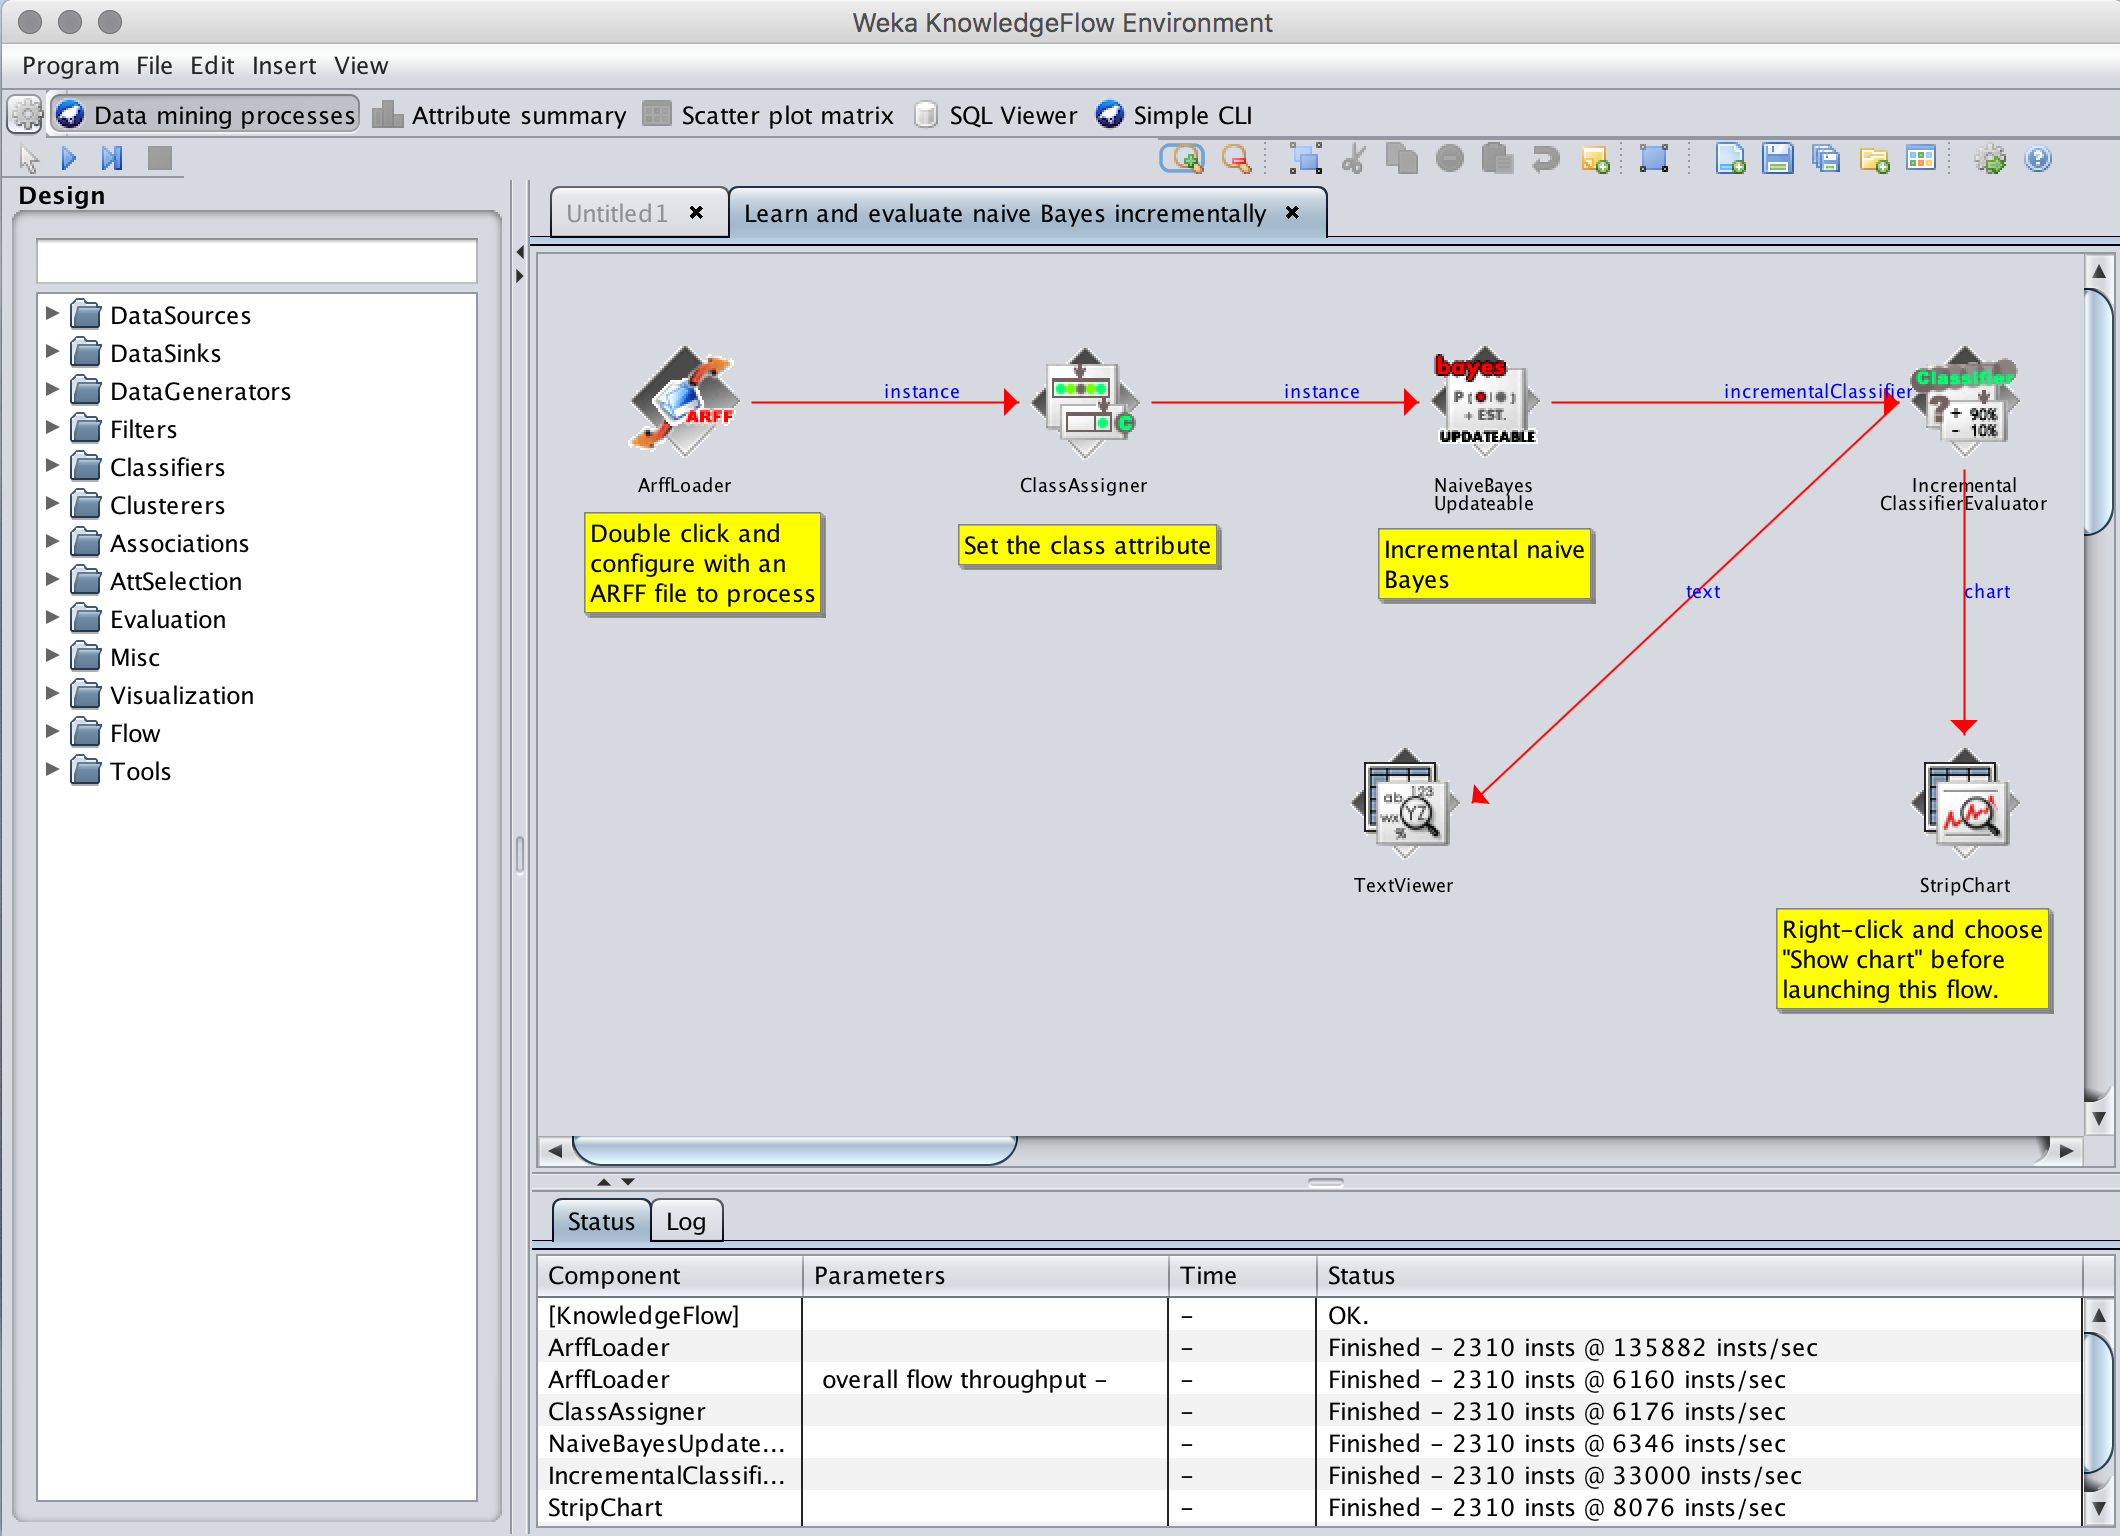
\includegraphics[width=0.85\textwidth]{images/B3_3a.png}}

\subfloat[\textit{StripChart} output.]{\label{subfig:kf_incremental_2}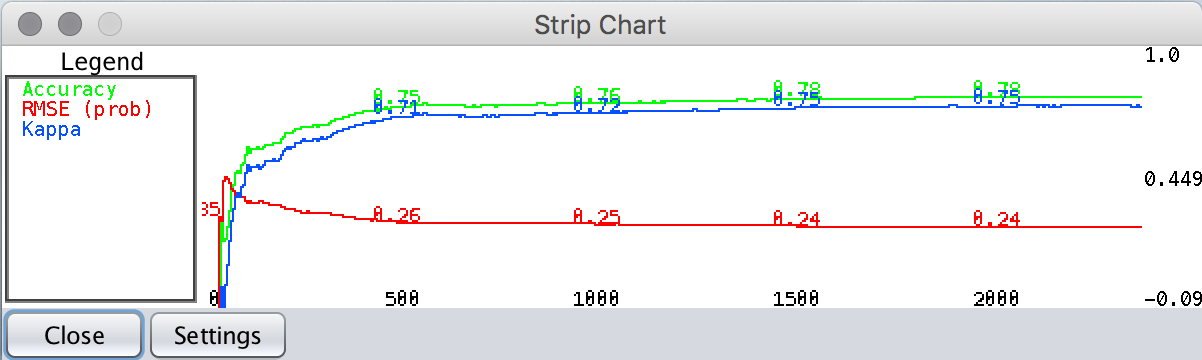
\includegraphics[width=0.85\textwidth]{images/B3_3b.png}}
\caption{\label{fig:kf_incremental}A Knowledge Flow that operates incrementally.}
\end{figure}

Figure~\ref{subfig:kf_incremental_1} shows a configuration that works incrementally. An
instance connection is made from the loader to a class assigner
component, which, in turn, is connected to the updatable Naive Bayes
classifier. The classifier's text output is taken to a viewer that
gives a textual description of the model. Also, an
\textit{incrementalClassifier} connection is made to the corresponding
performance evaluator. This produces an output of type \textit{chart},
which is piped to a \textit{StripChart} visualization component to
generate a scrolling data plot.

Figure~\ref{subfig:kf_incremental_2} shows the strip chart output. It
plots accuracy, Kappa, and the root mean-squared probability error
against time. As time passes, the whole plot (including the axes)
moves leftward to make room for new data at the right. When the
vertical axis representing time 0 can move left no farther, it stops
and the time origin starts to increase from 0 to keep pace with the
data coming in at the right. Thus when the chart is full it shows a
window of the most recent time units. The strip chart can be configured
to alter the number of instances shown on the $x$ axis.

This particular Knowledge Flow configuration can process input files
of any size, even ones that do not fit into the computer's main
memory. However, it all depends on how the classifier operates
internally. For example, although they are incremental, many
instance-based learners store the entire dataset internally.

